\begin{figure}
    \centering
    %Chart: Mean scores (Dimension 4)
    \begin{tikzpicture}
        \begin{axis}[
            axis lines=left,
            axis x line=bottom,
            axis line style={draw=black,-},
            width  = .85\textwidth,
            height = .25\textheight,
            major x tick style = transparent,
            ybar=3.0*\pgflinewidth,
            bar width=6pt,
            xmajorgrids = true,
            ymajorgrids = false,
            yticklabels={},
            ylabel = {\scriptsize Mean score},
            symbolic x coords={Professional letters,Press editorials,Romantic fiction,Hobbies,Personal letters,Interviews,General fiction,Telephone conversations,Prepared speeches,Spontaneous speeches,Religion,Official documents,Face-to-face conversations,Humor,Popular lore,Academic prose,Biographies,Mystery fiction,Press reportage,Science fiction,Adventure fiction,Press reviews,Broadcasts},
            xtick = data,
            nodes near coords,
            every node near coord/.append style={/pgf/number format/fixed},
            every node near coord/.append style={font=\tiny},
            every node near coord/.append style={rotate=90,anchor=west},
            nodes near coords style={/pgf/number format/.cd,precision=1},
            every axis/.append style={label style={font=\footnotesize},tick label style={font=\footnotesize}},
            x tick label style={rotate=30,anchor=east,font=\tiny,xshift=5pt},
            scaled y ticks = false,
            enlarge y limits={abs=.2*\pgfplotbarwidth},
            enlarge x limits={abs=1.5*\pgfplotbarwidth},
            extra y ticks = 0,
            extra y tick labels={},
            extra y tick style={grid=major,major grid style={thick,densely dashed,draw=red}}
        ]
        \addplot[style={draw=black,fill=red!50,mark=none}]
            coordinates {
                (Professional letters,3.5)
                (Press editorials,3.1)
                (Romantic fiction,1.8)
                (Hobbies,1.7)
                (Personal letters,1.5)
                (Interviews,1)
                (General fiction,.9)
                (Telephone conversations,.6)
                (Prepared speeches,.4)
                (Spontaneous speeches,.3)
                (Religion,.2)
                (Official documents,-.2)
                (Face-to-face conversations,-.3)
                (Humor,-.3)
                (Popular lore,-.3)
                (Academic prose,-.5)
                (Biographies,-.7)
                (Mystery fiction,-.7)
                (Press reportage,-.7)
                (Science fiction,-.7)
                (Adventure fiction,-1.2)
                (Press reviews,-2.8)
                (Broadcasts,-4.4)
            };
        \end{axis}
    \end{tikzpicture}
    \hspace*{12pt}
    %Chart: Loadings (Dimension 4)
    \begin{tikzpicture}
        \begin{axis}[
            axis lines=left,
            axis x line=bottom,
            axis line style={draw=black,-},
            width  = .85\textwidth,
            height = .25\textheight,
            major x tick style = transparent,
            ybar=3.0*\pgflinewidth,
            bar width=6pt,
            xmajorgrids = true,
            ymajorgrids = false,
            yticklabels={},
            ylabel = {\scriptsize Loading},
            symbolic x coords={Infinitives,Prediction modals,Suasive verbs,Conditional subordination,Necessity modals,Split auxiliaries,Possibility modals},
            xtick = data,
            nodes near coords,
            every node near coord/.append style={/pgf/number format/fixed},
            every node near coord/.append style={font=\tiny},
            every node near coord/.append style={rotate=90,anchor=west},
            nodes near coords style={/pgf/number format/.cd,precision=1},
            every axis/.append style={label style={font=\footnotesize},tick label style={font=\footnotesize}},
            x tick label style={rotate=45,anchor=east,font=\tiny,xshift=5pt},
            scaled y ticks = false,
            enlarge y limits={abs=.2*\pgfplotbarwidth},
            enlarge x limits={abs=1.5*\pgfplotbarwidth},
            extra y ticks = 0,
            extra y tick labels={},
            extra y tick style={grid=major,major grid style={thick,densely dashed,draw=red}}
        ]
        \addplot[style={draw=black,fill=blue!25,mark=none}]
            coordinates {
                (Infinitives,.76)
                (Prediction modals,.54)
                (Suasive verbs,.49)
                (Conditional subordination,.47)
                (Necessity modals,.46)
                (Split auxiliaries,.44)
                (Possibility modals,.37)
            };
        \end{axis}
    \end{tikzpicture}
    \caption{Dimensão 4 -- Expressão Explícita de Persuasão versus Não Explícita \citep[Original em língua inglesa]{biberVariationSpeechWriting1988}}
    \label{fig:merged_dim4_biber_ptbr}
\end{figure}
